\chapter{Redukcja argumentów}

Algorytm generowania indeksów zaproponowany przez profesora Sasao,
pozwala na zastosowanie pamięci o mniejszym rozmiarze niż wskazywałaby na to liczba argumentów.
Nie jest to oczywiście jedyna metoda pozwalająca na  uzyskanie takiego efektu.
W tej pracy przedstawione zostało podejście wykorzystujące jednocześnie redukcję i kompresję argumentów.

Redukcja argumentów jest to proces pozwalający na zmniejszenie liczby parametrów wejściowych funkcji poprzez odrzucenie argumentów zawierających wyłącznie redundantne dane.
Po wykonaniu takiego procesu,
usunięcie dowolnego argumentu z funkcji powoduje kolizję wierszy o różnych wartościach i tym samym utratę informacji.
Zbiór argumentów powstały w wyniku redukcji nazywamy reduktem.
Istnieje wiele sposobów redukcji argumentów,
zarówno systematycznych,
pozwalających na znalezienie wszystkich minimalnych rozwiązań,
jak i heurystycznych,
charakteryzujących się szybszym działaniem.
Sama redukcja nie zawsze przynosi spektakularne rezultaty.
W skrajnych przypadkach funkcji,
w których każdy argument dostarcza niewielkiej ale niezbędnej porcji informacji,
redukcja może nie przynieść żadnego efektu.
W takich przypadkach niezbędna jest,
opisana w dalszej części pracy,
kompresja argumentów,
świetnie sprawdzająca się właśnie w takich przypadkach.

\section{Problem złożoności}

Do problemu redukcji argumentów można podejść w sposób intuicyjny.
Można próbować po kolei usuwać argumenty i weryfikować spójność danych.
W przypadku utraty spójności taki argument musiałby się znaleźć w końcowym rozwiązaniu.
W przeciwnym przypadku należałoby go usunąć i kolejne weryfikacje przeprowadzać z jego wyłączeniem.
Pojedyncza weryfikacja wymaga porównania,
każdych dwóch wierszy o różnej wartości funkcji.
Jeżeli funkcja ma $n$ argumentów oraz $m$ wierszy wtedy porównanie dwóch dowolnych wierszy odbywa się ze złożonością liniową $n$.
Par wierszy do porównania jest w zależności od rozkładu wartości funkcji od $m$ do $m^2$.
Zatem złożoność obliczeniowa pojedynczej weryfikacji to $n \cdot m^2$.
Taką weryfikację trzeba przeprowadzić dla każdego z $n$ argumentów co daje końcową złożoność $n^2 \cdot m^2$.

Problem takiego podejścia,
poza złożonością,
leży dodatkowo w jakości uzyskiwanego rozwiązania.
W procesie redukcji argumentów,
część z nich może być ważniejsza i tym samym pozostawienie takiego argumentu może pozwolić na usunięcie dwóch (lub nawet więcej) innych.
Innymi słowami wynik takiej redukcji,
mimo że jest prawidłowy,
często jest nieoptymalny.

\section{Minimalne pokrycie kolumnowe}

Innym sposobem wyboru argumentów w czasie redukcji jest dobieranie argumentów,
aż do zapewnienia pełnej rozróżnialności.
Zaczynamy z jednym argumentem i kolejno wybieramy kolejne,
które znajdą się w końcowym rozwiązaniu.
Jeżeli przy takim podejściu dodatkowo będziemy w stanie ocenić,
które argumenty są bardziej wartościowe,
uzyskamy lepsze wyniki.

Za miarę wartości argumentu w redukcie można przyjąć liczbę rozróżnień,
których on dostarcza.
Jeżeli dzięki jednemu argumentowi jesteśmy w stanie rozróżnić tylko jedną parę wierszy o różnych wartościach to jest on mniej wartościowy od takiego,
który rozróżnia kilka par wierszy.
Z drugiej strony nawet argument,
który dostarcza jednego rozróżnienia,
będzie wartościowy jeżeli żaden inny go nie dostarcza.

Informacje o tych zależnościach uzyskuje się z macierz rozróżnialności, nazywana również tablicą porównań,
która zawiera wynik operacji XOR wszystkich par wierszy o różnych wartościach funkcji.
Jedynki w takiej macierzy obrazują,
które argumenty dostarczają jakich rozróżnień.

\begin{figure}[H]
\centering
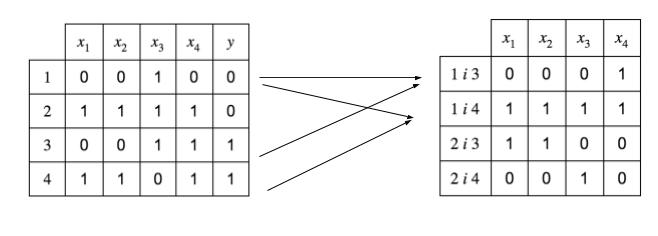
\includegraphics[width = 13cm]{chapter03/discernibility-table.jpg}
\caption{Proces powstawania tablicy rozróżnialności (Źródło własne).}
\end{figure}

Znalezienie reduktu,
przy użyciu tablicy rozróżnialności sprowadza się do problemu znalezienia minimalnego pokrycia kolumnowego,
czyli takiego zbioru kolumn,
dla którego w każdym z wierszy znajduje się co najmniej jedna jedynka.
Najprostszy algorytm znajdujący rozwiązanie sprowadzałby się do następujących kroków:
\begin{enumerate}
\item Wybranie kolumny o największej liczbie jedynek,
\item Usunięcie wierszy z jedynkami w tej kolumnie,
\item Powtarzanie aż do uzyskania pustej macierzy.
\end{enumerate}
Nie uwzględnia on jednak rozróżnień,
które są dostarczane przez niewielką liczbę argumentów.
Najłatwiej zauważyć to na przykładzie argumentów niezbędnych.
W ich przypadku istnieje taki wiersz,
który zawiera wyłącznie jedną jedynkę.
Oznacza to,
że argument odpowiadający tej jedynce jest niezbędny do uzyskania minimalnego pokrycia kolumnowego.
Taki argument często dostarcza innych rozróżnień,
które przy użyciu proponowanego algorytmu zawyżałyby sztucznie wartość innych argumentów.

\begin{figure}[H]
\centering
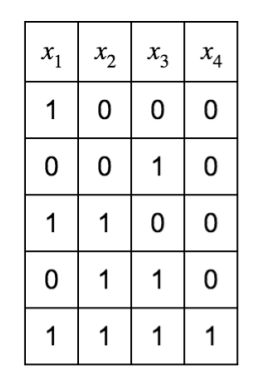
\includegraphics[width = 5cm]{chapter03/required-arguments.png}
\caption{Przykład obrazujący niedoskonałości algorytmu największej liczby jedynek. Argument $x_2$ posiada najwięcej jedynek i jednocześnie jest nadmiarowy. (Źródło własne).}
\end{figure}

Aby uwzględnić ten problem,
w ostatecznym rozwiązaniu sposób wyboru kolumny jest dwuetapowy.
Najpierw znajdowany jest wiersz o najmniejszej liczbie jedynek,
następnie wybierana jest kolumna,
która ma najwięcej jedynek oraz jedynkę w wybranym wierszu.
\textbf{Takie rozwiązanie wyboru kolumn jest optymalne i często prowadzi do uzyskania reduktu o najmniejszej liczności.}%TODO: CR:
Niestety w bardzo specyficznych przypadkach końcowe minimalne pokrycie kolumnowe również zawiera nadmiarowe argumenty.
Z tego powodu wymagane jest przeprowadzenie weryfikacji rozwiązania.


\begin{algorithm}[H]
    \KwData{$F$}
    \KwResult{$R$}
    $MR\gets$ pusta\;
    \For{dla każdej pary wierszy $F$ o różnej wartosci}{
        $W\gets$ wykonaj operację XOR poszczególnych bitów\;
        $MR\gets MR + W$\;
    }
    $MR2\gets MR$\;
    \While{$MR2$ nie pusta}{
        \For{dla każdego wiersza $MR2$}{
            $W\gets$ znajdź wiersz o najmniejszej liczbie jedynek\;
        }
        \For{dla kolumn z jedynekami w $W$}{
            $K\gets$ znajdź kolumnę o największej liczbie jedynek\;
        }
        $R\gets R + K$\;
        \For{dla każdego wiersza $W$ w $MR2$}{
            \If{$W$ zawiera jedynkę na $K$}{
                $MR2\gets MR2 - W$\;
            }
        }
    }
    \For{dla każdego argumentu $K$ w $R$}{
        \If{$MR$ dla argumentów z $R$ bez $K$ jest spójna}{
            $R\gets R - K$\;
        }
    }
\end{algorithm}

Dla takiej samej funkcji o $n$ argumentach i $m$ wierszach złożoność obliczeniowa tworzenia tablicy rozróżnialności wynosi $n \cdot m^2$.
Następne kroki algorytmu operują na macierzy rozróżnialności dlatego przy szacowaniu ich złożoności musimy pamiętać o tym,
że tablica ma $m^2$ wierszy.
Także kolejne złożoności znajdowania wiersza o najmniejszej liczbie jedynek oraz kolumny o największej liczbie jedynek wynoszą $n \cdot m^2$ każda.
Maksymalna liczba powtórzeń,
dla funkcji nieredukowalnej,
wynosi $n$.
Warto pamiętać,
że każdy kolejny krok jest wykonywany dla pomniejszonej liczby wierszy,
ale na potrzeby szacowania złożoności przyjmijmy skrajnie niekorzystny przykład,
gdzie każdy argument usuwa tylko po jednym wierszu.
W takim przypadku bardzo pesymistycznie oszacowana złożoność wyniesie $n^2 \cdot m^2$.
Ostatni krok ma taką złożoność jak poprzednio liczona złożoność weryfikacji.
Ponownie warto zauważyć,
że obliczenia przeprowadzane są już na redukcie,
czyli zbiorze argumentów często mniejszym od $n$.
Podsumowując końcowa złożoność obliczeniowa wynosi $n \cdot m^2 + n^2 \cdot m^2 + n^2 \cdot m^2$ czyli w dalszym ciągu $n^2 \cdot m^2$.
Wynika stąd,
że dzięki takiemu podejściu udało się uzyskać statystycznie lepszy redukt przy takiej samej złożoności obliczeniowej.


\section{Problem tablicy rozróżnialności}

W czasie przeprowadzania badań,
otrzymana złożoność nie stanowiła problemu.
Warto jednak zauważyć,
że rozmiar tablicy porównań dla bazy sygnatur wirusów o 1,3 mln wierszy,
byłby zbyt duży dla większości komputerów.
Jeżeli za rozmiar pojedynczego wiersza przyjęlibyśmy 5 bajtów (40 bitów), to o ile sama baza zajmowałaby ok 6 MB pamięci to tablica porównań ok 8 TB.

Taka złożoność pamięciowa jest niepraktyczna nie tylko w tym konkretnym przypadku,
ale również w wielu innych również poza domeną generowania indeksów.
Powstały z tego powodu algorytmy niewymagające generowania tablicy porównań.
Jednym z nich jest algorytm Marcina Korzenia i Szymona Jaroszewicza dokładnie przedstawiony w artykule “Finding Reducts Without Building the Discernibility Matrix”.

Przy zastosowaniu ich rozwiązania można policzyć liczbę jedynek w kolumnach tablicy rozróżnialności z praw kombinatoryki.
W artykule przedstawione zostały obliczenia dla bardzo ogólnej bazy danych,
jednak w ramach tej pracy,
istotny jest jedynie przypadek funkcji zawierającej wyłącznie zera i jedynki wśród wartości argumentów.
Jedynka w kolumnie macierzy rozróżnialności powstaje kiedy dwa wiersze o różnej wartości funkcji mają różną wartość argumentu.
Taka suma przy uwzględnieniu jedynie dwóch możliwych wartości argumentu i kilku wartości funkcji jest stosunkowo łatwa do wyznaczenia.
W przypadku ogólnym poruszanym w artykule jest jednak dużo łatwiej policzyć,
kiedy jedynka nie występuje w tablicy i odjąć tą liczbę od liczby wierszy w macierzy.
Dodatkowo,
ponieważ liczba wierszy jest identyczna dla każdej kolumny,
obliczanie liczby wierszy nie jest potrzebne.
Wystarczy zastosować odwrotne podejście przy wyborze kolumny i wybierać te o najmniejszej liczbie zer.

Jeżeli podzielimy wiersze danych na grupy ze względu na wartość funkcji i argumentu,
powstaną po dwa kubełki dla każdej wartości funkcji.
Jeżeli ich rozmiar oznaczymy $K_{0_d}$ i $K_{1_d}$,
 gdzie $0$ i $1$ oznaczają wartość argumentu,
a $d$ należy do zbioru wartości funkcji,
liczbę zer w kolumnie można wyrazić następującą sumą:
\begin{equation}
\sum_{0<d_1<d_2<D} K_{0_{d_1}} \cdot K_{0_{d_2}} + K_{1_{d_1}} \cdot K_{1_{d_2}}
\end{equation}
Obliczenie wyznacznika ma w takim wypadku złożoność pamięciową liniowo zależną od liczby wartości funkcji,
czyli pomijalnie małą.
Innymi słowy skutecznie rozwiązuje to problem pamięci zajmowanej przez tablicę rozróżnialności.
Dodatkowo mniejsza jest złożoność obliczeniowa.
Znalezienie najlepszej kolumny do uwzględnienia w redukcie odbywa się ze złożonością $n \cdot m$ w porównaniu do poprzedniego $n \cdot m^2$.

Takie rozwiązanie nie uwzględnia jednak argumentów niezbędnych i czasami będzie prowadzić do mniej optymalnych wyników niż algorytm użyty w niniejszej pracy.
Gdyby jednak dalsze badania lub konkretne zastosowania wymagały operacji na dużych bazach danych,
wymagane byłoby użycie tego lub podobnego algorytmu o mniejszej złożoności pamięciowej.

\section{Rozwiązania systematyczne}

Żadne z przedstawionych do tej pory rozwiązań nie było systematyczne.
Wszystko ze względu na zdecydowanie większą złożoność obliczeniową takich algorytmów.
W przypadku problemu generowania indeksów,
dane dla których przeprowadza się obliczenia zmieniają się w czasie,
dlatego czas tych obliczeń jest bardzo istotny.
Są jednak inne problemy,
w których czas optymalizacji nie jest czynnikiem istotnym.
Do takich zastosowań należą problemy dziedziny eksploracji danych,
gdzie często dane są zbierane na długo przed przeprowadzeniem obliczeń,
lub implementacji funkcji w układach FPGA czy też innych z pamięciami ROM.

W zadaniach, gdzie na wynik obliczeń możemy poczekać oraz nawet najmniejsza optymalizacja końcowego wyniku jest istotna,
rozwiązania systematyczne pokazują prawdziwą potęgę.
Na przykładzie redukcji argumentów,
takie algorytmy nie tylko dostarczają zawsze najmniejszy redukt,
ale wszystkie najmniejsze redukty.
Otwierają więc możliwość przeprowadzenia dalszych optymalizacji (np kompresji argumentów) z różnymi danymi początkowymi pozornie równie dobrymi.

\section{Unate Complement}

Ze względu na to,
że algorytmy systematyczne dostarczają wszystkich rozwiązań,
mogą w czasie badań służyć do weryfikacji jakości rozwiązań pochodzących z algorytmów heurystycznych.
Algorytmem użytym w tym celu w ramach pracy był algorytm Unate Complement.

Algorytm Unate Complement służy do wyznaczania dopełnienia funkcji jednorodnej,
czyli takiej,
dla której w żadnej kolumnie nie występują jednocześnie zera i jedynki.
Tym samym pozwala na znalezienie wszystkich największych (najbardziej ogólnych) kostek dopełnienia funkcji jednorodnej,
a zastosowany do tablicy porównań pozwala na wyznaczenie wszystkich minimalnych pokryć kolumnowych.

Sam algorytm składa się z czterech kroków:
\begin{enumerate}
\item Rekurencyjnego rozkładu funkcji zgodnie ze wzorem Shannona,
\item Obliczania dopełnień w liściach zgodnie z prawami De Morgana,
\item Rekurencyjnego łączenia powstałych dopełnień ponownie przy wykorzystaniu wzoru Shannona,
\item Usunięcia nadmiarowych reduktów,
czyli takich które zawierają się w innych zgodnie z rachunkiem kostek.
\end{enumerate}
Badania nad tym algorytmem zostały opisane w pracy inżynierskiej \cite{inzynierka},
a gotowy program służył do weryfikacji poprawności działania użytego algorytmu redukcji argumentów.
